\chapter{Evaluation and Experiments}
\todo{fix formatting mess}
This chapter describes the evaluation methodology and outlines the metrics and figures that we used to quantify the performance of our learned policies on both single-quadrotor and multi-quadrotor cable-suspended payload transport tasks.

\section{Experimental Setup}
We first evaluate the performance of our learned policies in our simulation environment. We use only the actor network for evaluation, as the critic is not needed. The policies are trained using the \gls{ippo} algorithm.  
All experiments were conducted in simulation using a policy frequency of 250~Hz with one physics step per control action. We set both observation and actuator noise to zero, randomized thrust within 80--100\% thrust range, used a 0.3~m cable length, and fixed the payload mass at 0.01~kg.

Two primary tasks were evaluated: the recovery-from-harsh-conditions task and the figure-eight trajectory tracking task. The recovery task involved stabilizing the payload at a target position after being disturbed, while the trajectory tracking task required the quadrotor to follow a precomputed figure-eight path while keeping the payload stable.

In the recovery task, episodes lasted 2,500 steps, the payload target remained fixed at $(0,0,1.5)$~m, and the agent began from random harsh initial states. The payload and quadrotor positions as well as the quadrotors' orientations and velocities are randomized. Metrics were gathered over 1,000 rollouts. We evaluate the specific policies for single quadrotor with payload; teams of two, three, and six quadrotors were evaluated, each initialized as described in section~X\todo{ref}. The payload was always initialized at $(0,0,1.5)$~m, and the quadrotors were positioned randomly in a half-sphere around it. It's important to note that this includes different cable modes, with sometimes the cable being slack and sometimes taut, forcing the quadrotor to stabilize the payload in all modes. These states emulate the state after a strong disturbance, like a collision with an obstacle or the quadrotors being thrown into the air.

In the figure-eight tracking task, each episode ran for 5,000 steps simulating 20~s, the payload has to follow a precomputed figure-eight path, and the quadrotor is always initialized at the center with quads in random positions, with performance aggregated over 100 rollouts.

\section{Single-Quadrotor Payload Control}
We first evaluate the learned policy on the single-vehicle case, testing both harsh condition recovery and trajectory tracking on a figure-eight path. We run each with a policy trained specifically for the single quadrotor with payload scenario. The results are shown in Figure~\ref{fig:payload_error_over_time_single} and Figure~\ref{fig:one_recovery}.
Figure~\ref{fig:one_recovery} shows some example runs of the recovery task, where the quadrotor is initialized in random states and has to stabilize the payload at the target position $(0,0,1.5)$~m. The quadrotor successfully stabilizes the payload within 2~s for most initial conditions. In the figure, the bottom two runs labeled 6 and 7 show takeoff from the ground, which is hard due to a very sudden mode switch from slack to taut cable close to the ground. Runs 1 to 5 show the active swing counteraction of the quadrotor, where it actively stabilizes the payload on the path to the target. Runs 3 and 4 specifically show a very strong initial payload swing. All runs stabilize the payload swing before reaching the target position without any oscillations or overshoot. They then stabilize there without much movement for the rest of the run. We can see that the policy generalizes to all relative positions of the payload to the target and the quadrotor to the payload. During recovery the payload reaches speeds of up to 1.7~m/s, highlighting the learned agility of the policy. If this level of agility is not desired, the speed can be reduced by adjusting the linear velocity components of the reward function.

We here only show recovery from up to 1.5~m. This, though, generalizes to any distance by clipping the length of the position error vector to 1~m. Additionally to the qualitative analysis, we also show a more thorough statistical analysis in Figure~\ref{fig:payload_error_over_time_single}. Here we statistically evaluate 1,000 recovery runs from harsh conditions. The termination histogram shows that 99\% of harsh initial conditions are recovered successfully, while the remaining terminate right in the beginning due to very harsh initialization. The position error over time also shows that we recover from distances of up to 1~m in roughly 2~s. It also shows that all runs stably hover at the target for over 5~s after reaching it.

To show that the position tracking capabilities generalize to a moving setpoint, we evaluate on a precomputed figure-eight trajectory. For each timestep we sample the policy position setpoint on the figure-eight trajectory, leading to the tracking behavior shown in Figure~\ref{fig:one_eight}. The figure shows the path of 5 runs randomly initialized around the start point of the trajectory, with the quads in suboptimal states. The figure shows how the quads very quickly manage to stabilize themselves and then continue after around 3~s to accurately follow the trajectory. Even though all quads are initialized with slightly different thrust ranges they all manage to accurately track the correct height of the trajectory. Due to the policy currently just being able to do position tracking, it always slightly lags behind the trajectory. This can be seen at the end of the trajectory where it does not fully reach the center. This could be reduced by explicitly training on trajectory following and adding multiple trajectory points or velocity states as shown in previous work.

These experiments show that the trained policy for the single quadrotor with payload case exhibits great payload swing stabilization ability, while also being agile and very accurate in tracking.

\begin{figure}[H]
  \centering
  % first row
  \begin{subfigure}[t]{0.49\textwidth}
    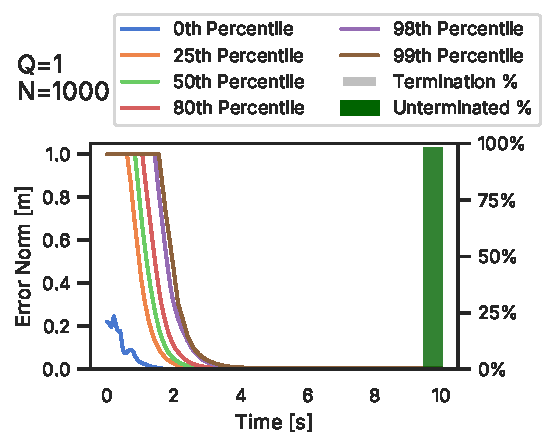
\includegraphics[width=\textwidth]{experiments/one_recovery_error.pdf}
    \caption[Single quadrotor recovery evaluation]{Recovery in the single quadrotor with payload scenario from 1000 different initial harsh states. The Percentiles show smooth reduction of the initial high tracking error converging to 0. The termination percentatge shows that most runs are successful and not terminated.}
    \label{fig:payload_error_over_time_single}
  \end{subfigure}\hfill
  \begin{subfigure}[t]{0.49\textwidth}
    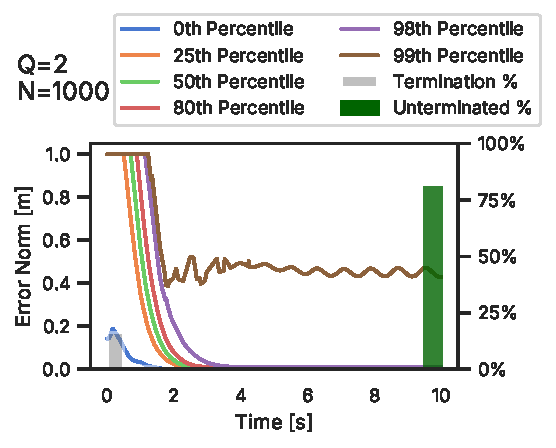
\includegraphics[width=\textwidth]{experiments/two_recovery_error.pdf}
    \caption[Two quadrotor recovery evaluation]{Recovery in the two quadrotor with payload scenario from 1000 different initial harsh states. The Percentiles show smooth reduction of the initial high tracking error for most inital harsh states evantually converging to 0. The termination percentage shows that a high number of runs are successful and not terminated while most terminations occur right at initialization, because of very harsh initialization.}
    \label{fig:payload_error_over_time_two}
  \end{subfigure}

  \vspace{1em}  % optional space between rows
  % second row
  \begin{subfigure}[t]{0.49\textwidth}
    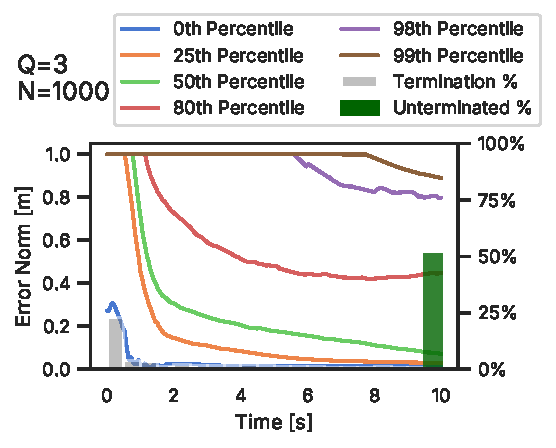
\includegraphics[width=\textwidth]{experiments/three_recovery_error.pdf}
    \caption[Three quadrotor recovery evaluation]{Recovery in the three quadrotor with payload scenario from 1000 different initial harsh states. The Percentiles show smooth reduction of the initial high tracking error converging to 0. The termination percentage shows that nearly all runs are successful and not terminated, while most terminations occur right at initialization, because of very harsh initialization.}
    \label{fig:payload_error_over_time_three}
  \end{subfigure}\hfill
  \begin{subfigure}[t]{0.49\textwidth}
    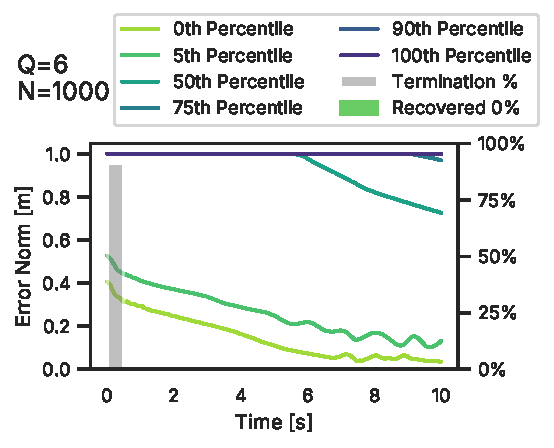
\includegraphics[width=\textwidth]{experiments/six_recovery_error.pdf}
    \caption[Six quadrotor recovery evaluation]{Recovery in the six quadrotor with payload scenario from 1000 different initial harsh states. Most runs are terminated early, indicating limits of the approach.}
    \label{fig:payload_error_over_time_six}
  \end{subfigure}

  \caption[Recovery error comparison]{Recovery error over time for different quadrotor configurations with payload. The lines show the distance percentiles of the unterminated runs at each timestep. The green bar indicates the percentage of runs that were successfully recovered and stabilized at the target. The gray bars show the frequency of terminations over time.}
  \label{fig:single_quad_payload_subfigs}
\end{figure}



\begin{figure}[H]
    \centering
    
    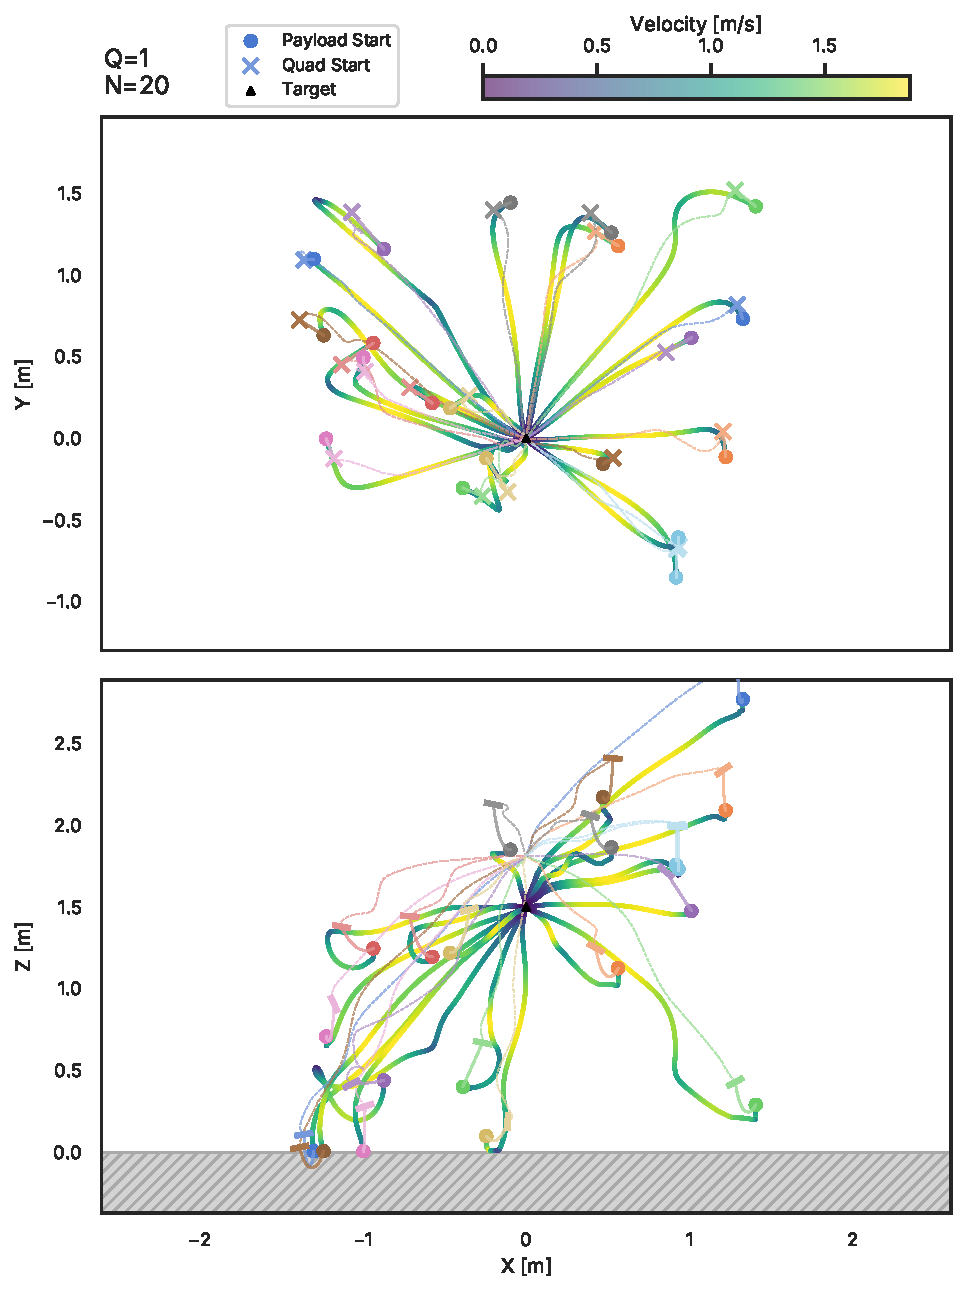
\includegraphics[width=\textwidth]{experiments/one_recovery.pdf}
    \caption[Single quadrotor harsh recovery trajectory]{Recovery of one quadrotor with payload from harsh conditions. The top plot is top-down  (xy) view, while the bottom one is side view (xz).
    The figure shows N=8 runs. The position is initialized randomly and the goal is to recover to the target and stabilize. The quadrotor successfully stabilizes the payload within 2 seconds. The initial states of the quadrotor and payload are marked and labeled with their run id. The cables are drawn to represent their mode and cable length, slackness in the cable being shown as a curve.}
    \label{fig:one_recovery}
\end{figure}
\begin{figure}[H]
    \centering
    
    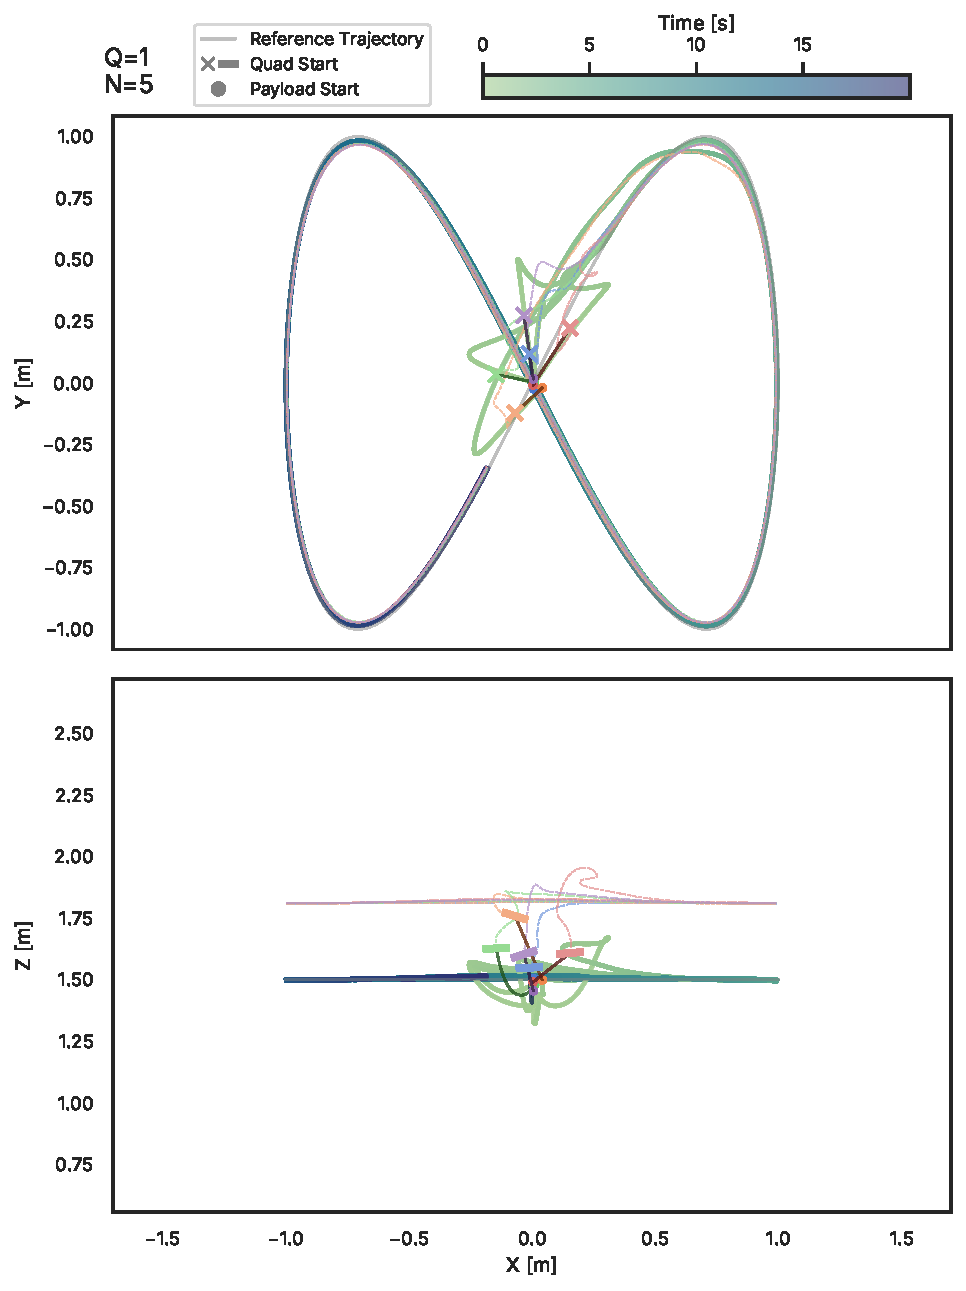
\includegraphics[width=\textwidth]{experiments/one_eight.pdf}
    \caption[Single quadrotor figure-eight tracking]{Figure-eight trajectory tracking for one quadrotor with payload.The top plot is top-down  (xy) view, while the bottom one is side view (xz). The figure shows N=5 runs. The position is initialized near the target with random quadrotor states. The quadrotor successfully follows the figure-eight path while stabilizing the payload.}
    \label{fig:one_eight}
\end{figure}

\section{Multi-Quadrotor Payload Transport}
We extend the evaluation to cooperative transport tasks involving teams of two and three quadrotors to show learned coordinated behavior. The simulation configuration and scenarios are set up similarly to the single-quadrotor case, with the payload always initialized at $(0,0,1.5)$~m and the quadrotors positioned randomly in a half-sphere around it as described in section~\ref{sec:reset}. The policies are trained specifically for the number of quadrotors in the team. For three quadrotors we increase the payload mass to 20~g to ensure that the payload is heavy enough to require cooperation. The policies are trained using the \gls{ippo} algorithm with the same hyperparameters as in the single-quadrotor case.

\subsection{Two Quadrotors}
We first evaluate the learned policy on the two-quadrotor case, testing both harsh condition recovery and trajectory tracking on a figure-eight path. We run each with the policy trained specifically for the two quadrotor with payload scenario. The results are shown in Figure~\ref{fig:payload_error_over_time_two}, Figure~\ref{fig:two_recovery} and Figure~\ref{fig:two_eight}.

Figure~\ref{fig:two_recovery} shows some example runs of the recovery task, where the quadrotors and payload are initialized in random states and have to stabilize the payload at the target position. The runs labeled 0 and 1 show successful takeoff. 4 and 3 show stabilization of swinging payload. 4 in specific shows a very harsh tilt orientation of the quadrotor that is recovered from. 3 to 7 are all initialized with slack cables. The payload is stabilized at the target within 2~s, moving at speeds of up to 1.5~m/s. The quadrotors then stabilize the payload at the target position without oscillations or overshoot.
We also evaluate this in Figure~\ref{fig:payload_error_over_time_two}, where we statistically evaluate 1,000 recovery runs from harsh conditions. The termination histogram shows that 81\% of harsh initial conditions are recovered successfully, while the remaining terminate mostly in the beginning due to very harsh initialization. The position error over time also shows that we recover from distances of up to 1~m in roughly 2~s. It also shows that all runs stably hover at the target for over 5~s after reaching it. Some of the failed runs struggle to recover and get stuck in an oscillation leading to termination. This is due to very harsh initialization, leading to the quadrotors running into each other right after initialization. This can be improved by better initialization of the quadrotors and payload, which is discussed in section~\ref{sec:reset}.

To show that the position tracking capabilities generalize to a moving setpoint we evaluate on a precomputed figure-eight trajectory. We use the same setup as with the single-quad case. We show the results in Figure~\ref{fig:two_eight}. The figure shows the path of 5 runs randomly initialized around the start point of the trajectory, with the quads in suboptimal states. The figure shows how the quads very quickly manage to stabilize themselves and then continue after around 3~s to follow the trajectory. The tracking is a bit less accurate than the single-quad case, but still shows good performance. Even though all quads are initialized with slightly different thrust ranges they all manage to accurately track the correct height of the trajectory. We might further improve the tracking performance by explicitly training on trajectory following and adding multiple trajectory points or velocity states as shown in previous work and also adding the velocity state of the other quadrotors to the observation space.
\begin{figure}[H]
    \centering
    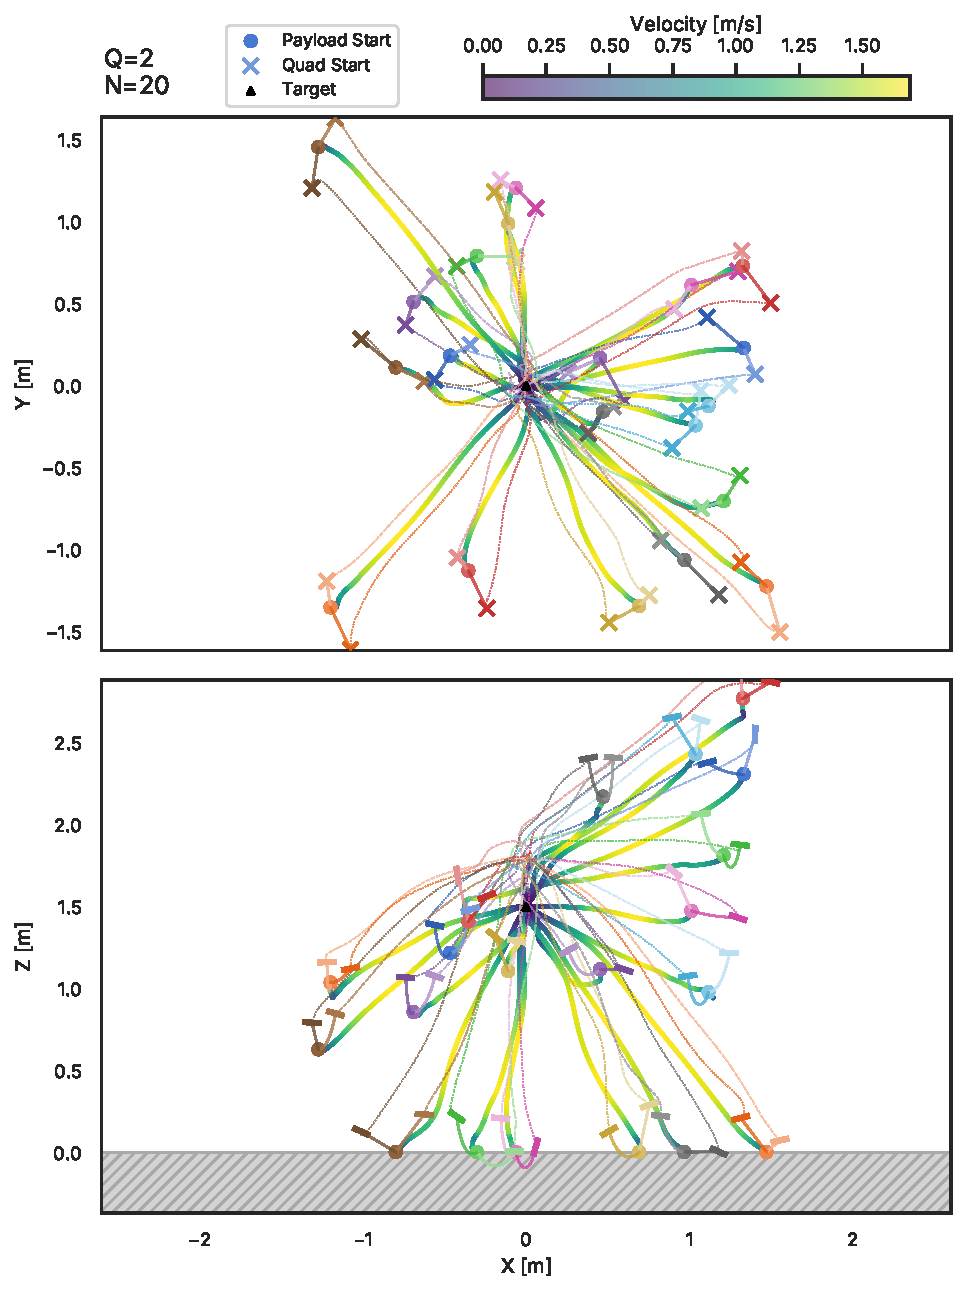
\includegraphics[width=\textwidth]{experiments/two_recovery.pdf}
    \caption[Two quadrotor harsh recovery trajectory]{Recovery of two quadrotors with payload from harsh conditions. The top plot is top-down  (xy) view, while the bottom one is side view (xz).
    The figure shows N=8 runs. The position of payload and quadrotors is initialized randomly and the goal is to recover to the target and stabilize. The quadrotor successfully stabilizes the payload within 2 seconds. The initial states of the quadrotor and payload are marked and labeled with their run id. The cables are drawn to represent their mode and cable length, slackness in the cable being shown as a curve.}
    \label{fig:two_recovery}
\end{figure}
\begin{figure}[H]
    \centering
    
    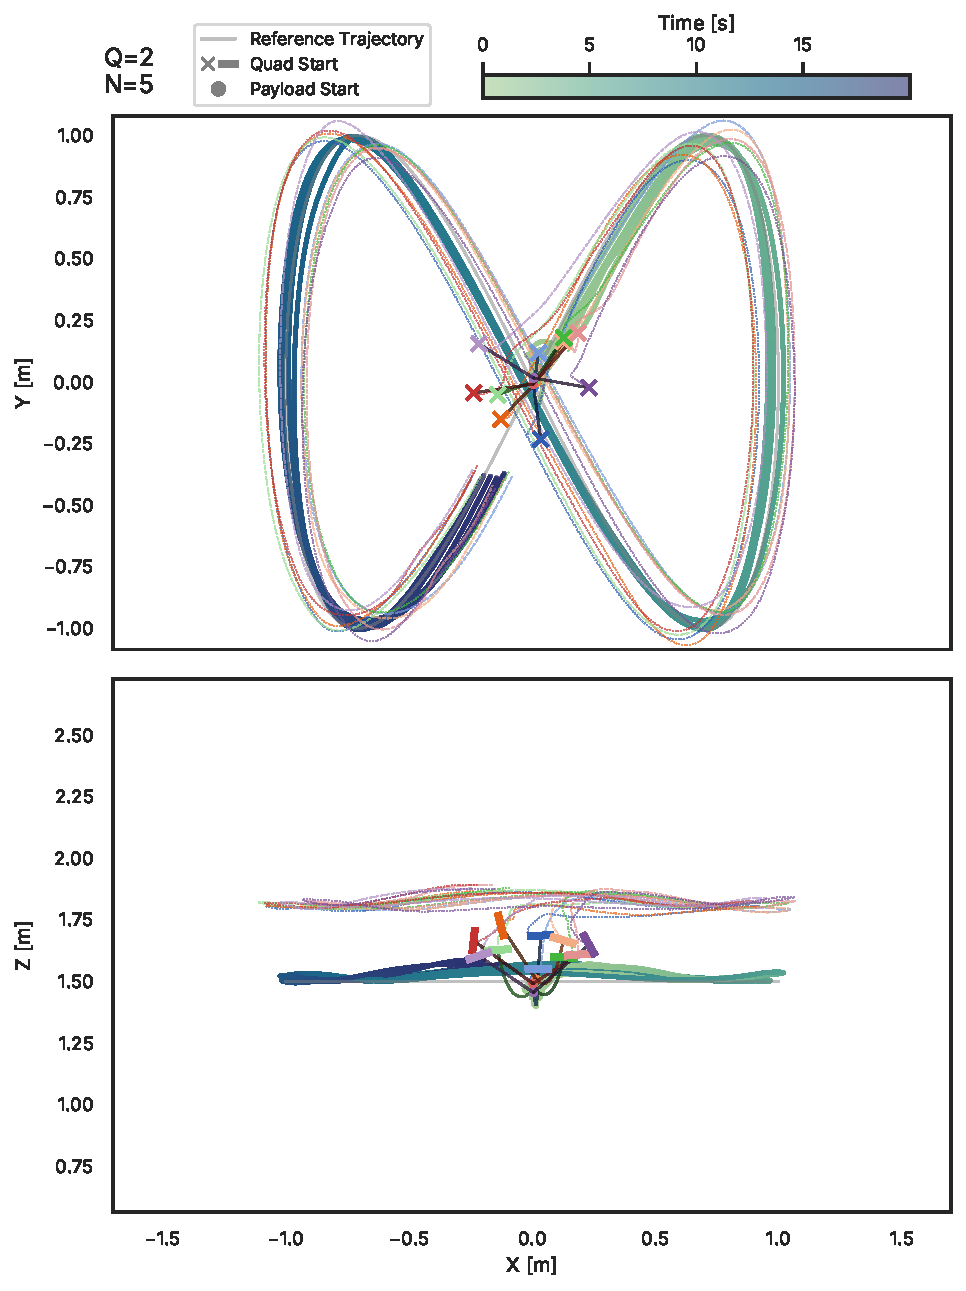
\includegraphics[width=\textwidth]{experiments/two_eight.pdf}
    \caption[Two quadrotor figure-eight tracking]{Figure-eight trajectory tracking for two quadrotors with payload.The top plot is top-down  (xy) view, while the bottom one is side view (xz). The figure shows N=5 runs. The position is initialized near the target with random quadrotor states. The quadrotor successfully follows the figure-eight path while stabilizing the payload.}
    \label{fig:two_eight}
\end{figure}
\subsection{Three Quadrotors}
We extend the evaluation to three quadrotors, testing both harsh condition recovery and trajectory tracking on a figure-eight path. We run each with the policy trained specifically for the three quadrotor with payload scenario. The results are shown in Figure~\ref{fig:three_recovery} and Figure~\ref{fig:three_eight}. The policies are trained using the \gls{ippo} algorithm with the same hyperparameters as in the single-quadrotor case, but with a payload mass of 20~g to ensure that the payload is heavy enough to require cooperation.

Figure~\ref{fig:three_recovery} shows some example runs of the recovery task, where the quadrotors and payload are initialized in random states and have to stabilize the payload at the target position. The payload is stabilized at the target within 2~s, moving at speeds of up to 1.5~m/s. The quadrotors then stabilize the payload at the target position without oscillations or overshoot.

We also evaluate this in Figure~\ref{fig:payload_error_over_time_three}, where we statistically evaluate 1,000 recovery runs from harsh conditions. The termination histogram shows that 99\% of harsh initial conditions are recovered successfully, while the remaining terminate mostly in the beginning due to very harsh initialization. The position error over time also shows that we recover from distances of up to 1~m in roughly 2~s. It also shows that all runs stably hover at the target for over 5~s after reaching it. Some of the failed runs struggle to recover and get stuck in an oscillation leading to termination. This is due to very harsh initialization, leading to the quadrotors running into each other right after initialization. This can be improved by better initialization of the quadrotors and payload, which is discussed in section~\ref{sec:reset}.

\begin{figure}[H]
    \centering
    
    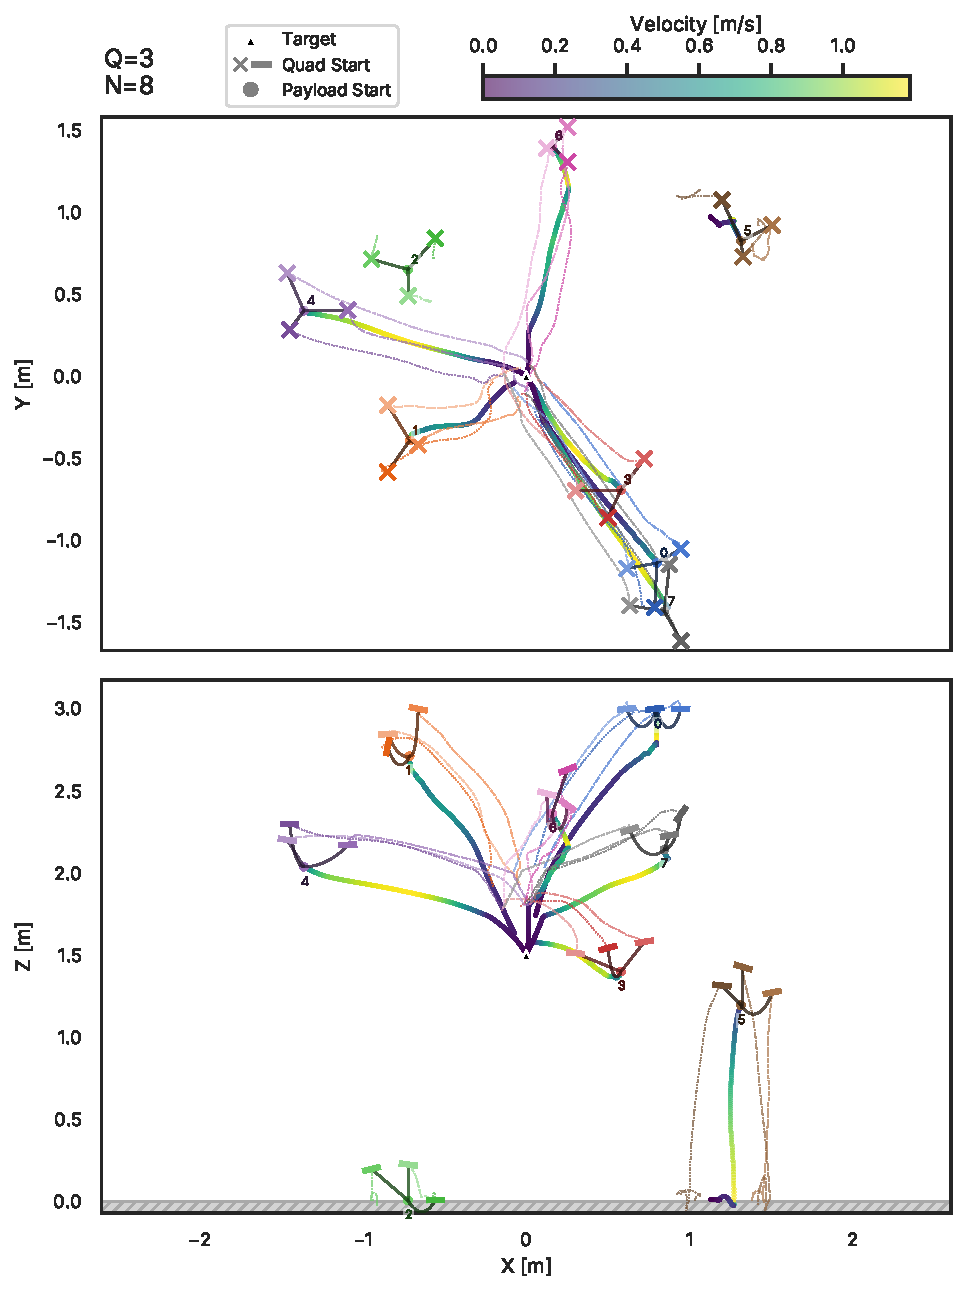
\includegraphics[width=\textwidth]{experiments/three_recovery.pdf}
    \caption[Three quadrotor harsh recovery trajectory]{Recovery of three quadrotors with payload from harsh conditions. The top plot is top-down  (xy) view, while the bottom one is side view (xz).
    The figure shows N=8 runs. The position of payload and quadrotors is initialized randomly and the goal is to recover to the target and stabilize. The quadrotor successfully stabilizes the payload within 2 seconds. The initial states of the quadrotor and payload are marked and labeled with their run id. The cables are drawn to represent their mode and cable length, slackness in the cable being shown as a curve.}
    \label{fig:three_recovery}
\end{figure}
\begin{figure}[H]
    \centering
    
    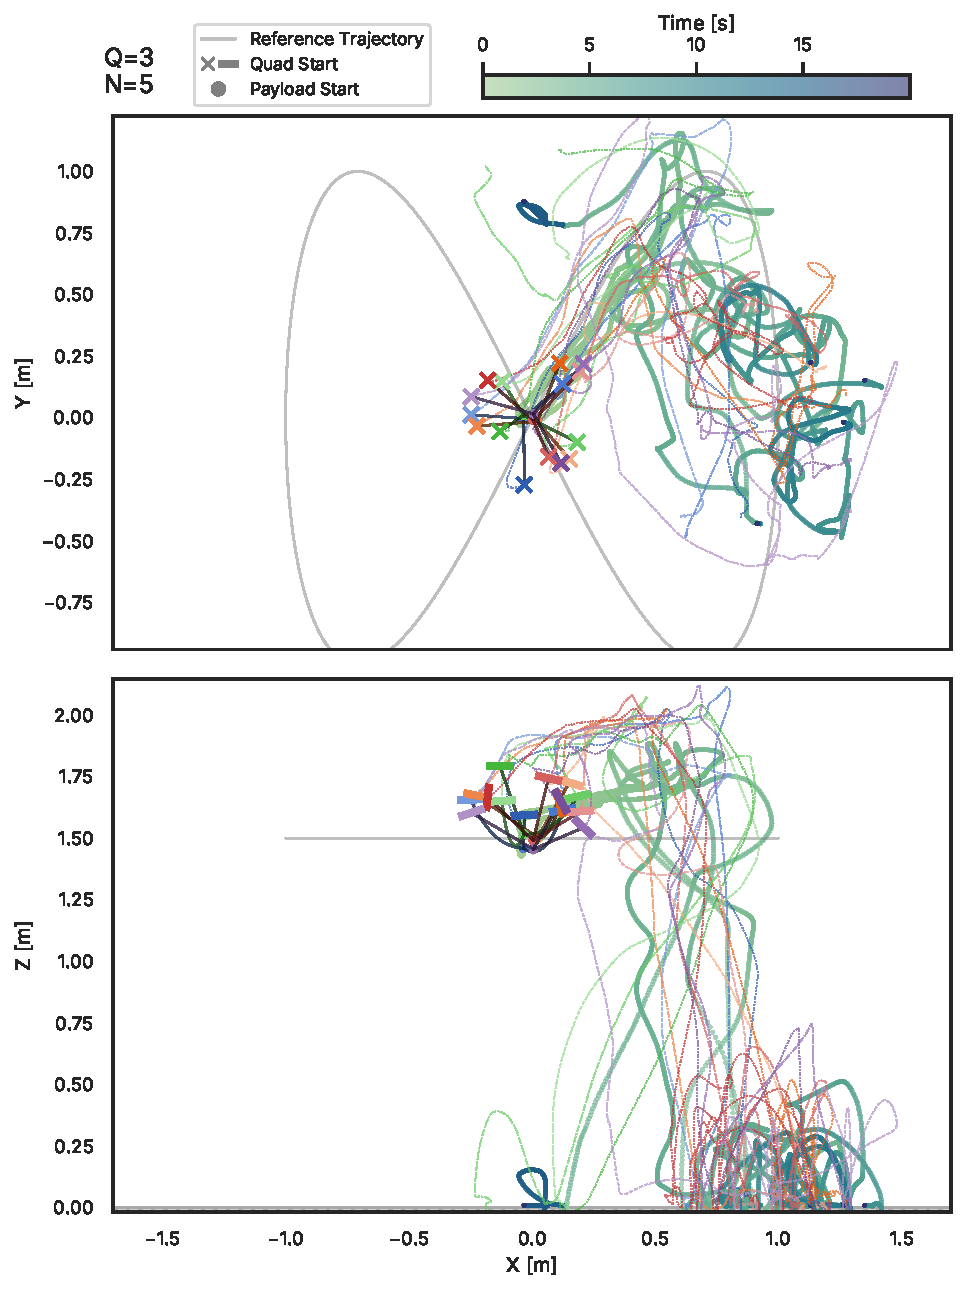
\includegraphics[width=\textwidth]{experiments/three_eight.pdf}
    \caption[Three quadrotor figure-eight tracking]{Figure-eight trajectory tracking for three quadrotors with payload.The top plot is top-down  (xy) view, while the bottom one is side view (xz). The figure shows N=5 runs. The position is initialized near the target with random quadrotor states. The quadrotor successfully follows the figure-eight path while stabilizing the payload.}
    \label{fig:three_eight}
\end{figure}

\subsection{Six Quadrotors}
The last configuration we evaluate is a team of six quadrotors, testing recovery from harsh conditions to evaluate the scalability of our approach. We run them with the policy trained specifically for the six quadrotor with payload scenario. The results are shown in Figure~\ref{fig:payload_error_over_time_six} evaluating 1,000 runs on the recovery scenario.

The policies are trained using the \gls{ippo} algorithm with the same hyperparameters as in the single-quadrotor case, but with a payload mass of 40~g to ensure that the payload is heavy enough to require cooperation.  
The termination histogram in Figure~\ref{fig:payload_error_over_time_six} shows that most runs are terminated early indicating limits of our approach. These terminations mostly happen because the quadrotors struggle to coordinate their movements effectively under the increased complexity of the scenario, leading to collisions. A major limitation of our approach is that we currently do not preprocess or sort the other quadrotors' positions in the observation space, which leads to the policy not being able to effectively coordinate the movements of the quadrotors, because it needs to cover all possible combinations of relative positions. 

One possible solution to this could be to sort the other quadrotors' positions by their distance to the agent in the observations, to reduce the complexity.
Other approaches, that future work could investigate to improve on these limitations include privileged critic approaches, better representation of the payload and quadrotors in the observation space, and more complex network architectures, like for example utilizing attention architectures as in \autocite{huang_collision_2024}.

\section{Comparison with Baseline}
\begin{figure}[H]
    \centering
    
    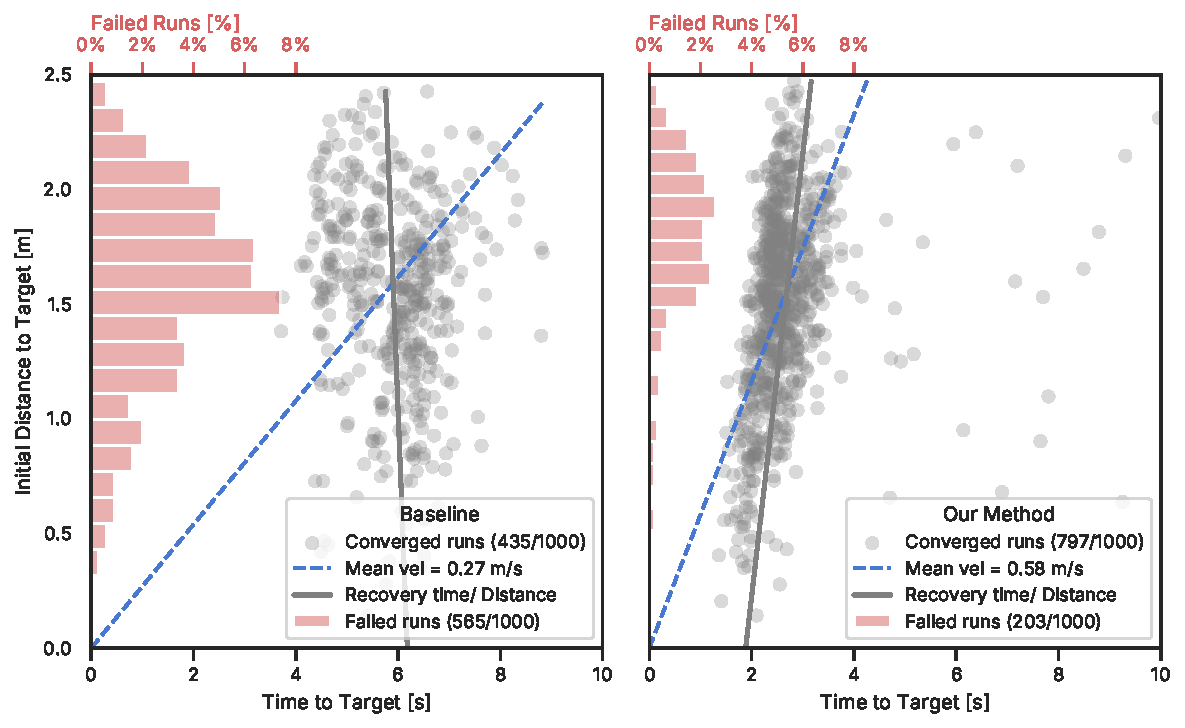
\includegraphics[width=\textwidth]{experiments/baseline_stat_comparison.pdf}
    \caption[Baseline vs RL Performance]{Comparison of the learned policy with the baseline method from \autocite{Wahba2024}. We compared the methods on N=1000 runs initialized in harsh conditions. The left plot shows the the baseline method. The right plot shows the learned policy. Our method achieves a significantly lower error recovery time and failure rate.}
    \label{fig:baseline_histogram_comparison}

\end{figure}
\todo{fix baseline comparison}
We compare our learned policy with the baseline method from \autocite{Wahba2024} in terms of recovery from harsh conditions performance. The baseline planner models each cable as a rigid rod and relies on centralized offline trajectory optimization with an online controller that tracks these precomputed paths, which limits its ability to capture cable swing and mode switching, adapt to unexpected disturbances or payload changes or collisions, and meet real-time computational demands. Our Method adresses these limitations by leveraging reinforcement learning for a more robust decentalized solution.

We compare our method with the baseline on the two quadrotor with payload scenario, where we evaluate the recovery from harsh conditions. We initialize the payload at $(0,0,1.5)$~m and the quadrotors in random positions around it. The baseline method is run with the same initialization and the same target position. We evaluate both methods on 1000 runs each, with the payload initialized in random states and the quadrotors in random positions around it. 

The results are shown in Figure~\ref{fig:baseline_recovery} and Figure~\ref{fig:baseline_histogram_comparison}.
Figure~\ref{fig:baseline_histogram_comparison} shows significantly higher recovery rates of 80\% with our method compared to 19\% with the baseline method. Also we can see that our method achieves a significantly lower static position error of a mean 0.5cm compared to a mean of 2.9cm with the baseline method. The baseline method fails to recover from harsh conditions in most cases, while our method is able to recover from most initial conditions and stabilize the payload at the target position.

Figure~\ref{fig:baseline_recovery} also shows the qualitative difference of the trajectories in the recovery task, where the quadrotors and payload are initialized in random states and have to stabilize the payload at the target position. Most runs fail with the baseline method while our method manages to stabilize at the target. The runs labeled 0 and 1 show successful recoveries of the baseline method. Here it is also shown that our method achieves a more efficient straight line trajectory to the target position, while the baseline method goes through a more complex trajectory spiraling to the target.

It is important to note that the baseline method might perform better in some specific scenarios, especially when the payload is in a very stable state and the quadrotors are in optimal positions. However, our method shows a more robust performance across a wider range of initial conditions and disturbances, making it more suitable for real-world applications where such conditions are common. Also our method currently does not take obstacles into account, which is a limitation of the current approach. Future work could extend our method or combine it with the motion planning of the baseline method to achieve obstacle avoidance capabilities. \todo{mention no simtoreal}

\begin{figure}[H]
    \centering
    
    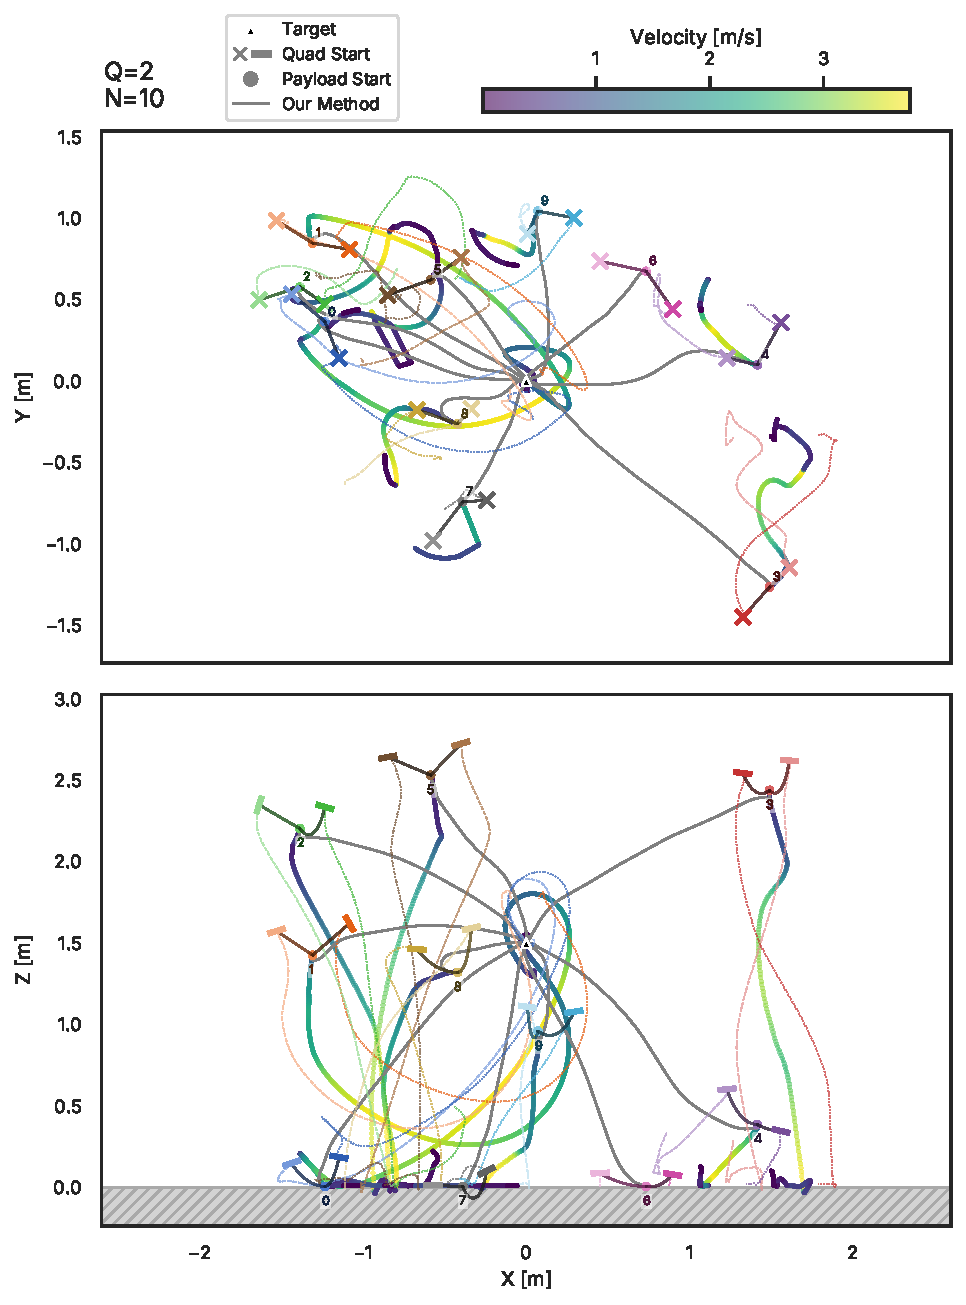
\includegraphics[width=\textwidth]{experiments/baseline_recovery.pdf}
    \caption[Baseline vs learned two quad recovery]{Comparison of the learned policy with the baseline method from \autocite{Wahba2024}. Recovery of two quadrotors with payload from harsh conditions. The top plot is top-down  (xy) view, while the bottom one is side view (xz).}
    \label{fig:baseline_recovery}
\end{figure}

% \section{Sim-to-Real Transfer}
% - one and three quads  
% - Plots Traj: Trajectory following 3d, error over time  
% - Plots Disturbance: Position holding with disturbance  

\section{Generalization}
Does it generalize to different payloads and cable lengths?\todo{Generalization section}

\section{Experimental Results Summary}
In this chapter, we evaluated the performance of our learned policies in both single-quadrotor and multi-quadrotor scenarios. The results demonstrate that our approach effectively stabilizes payloads in harsh conditions and accurately tracks trajectories. The policies generalize well to different initial conditions and quad configurations. We also showed that the approach scales to teams of up to six quadrotors, with the policy being able to recover from harsh conditions and stabilize the payload at the target position. We compared our method with existing baselines and demonstrated its superiority in terms of stability and robustness. Overall, our approach provides a robust solution for cooperative aerial transport tasks, demonstrating the potential of reinforcement learning in this domain.